% Figure 5.5 (Session 5): acting with H on a matrix product state, and the DMRG sweep.
% The image is rendered by figures/blender/s5_5_mps_algorithm.py; the coordinates of the labels
% come from figures/blender/out/mps_algorithm_anchors.tex. Built by figures/blender/build_figure.sh.
\documentclass[11pt,tikz,border=0pt]{standalone}
\usepackage{amsmath,amssymb,graphicx,braket}
\usepackage{xcolor}
\definecolor{coursedark}{HTML}{1B2A4A}
\definecolor{costamber}{HTML}{B8620A}
\newlength{\figw}\setlength{\figw}{16.19cm}   % the text width of the notes (letter, 2.7 cm margins), so labels print at size

\begin{document}
\begin{tikzpicture}[lbl/.style={font=\small, text=coursedark}]
  \node[anchor=south west, inner sep=0pt] at (0,0)
    {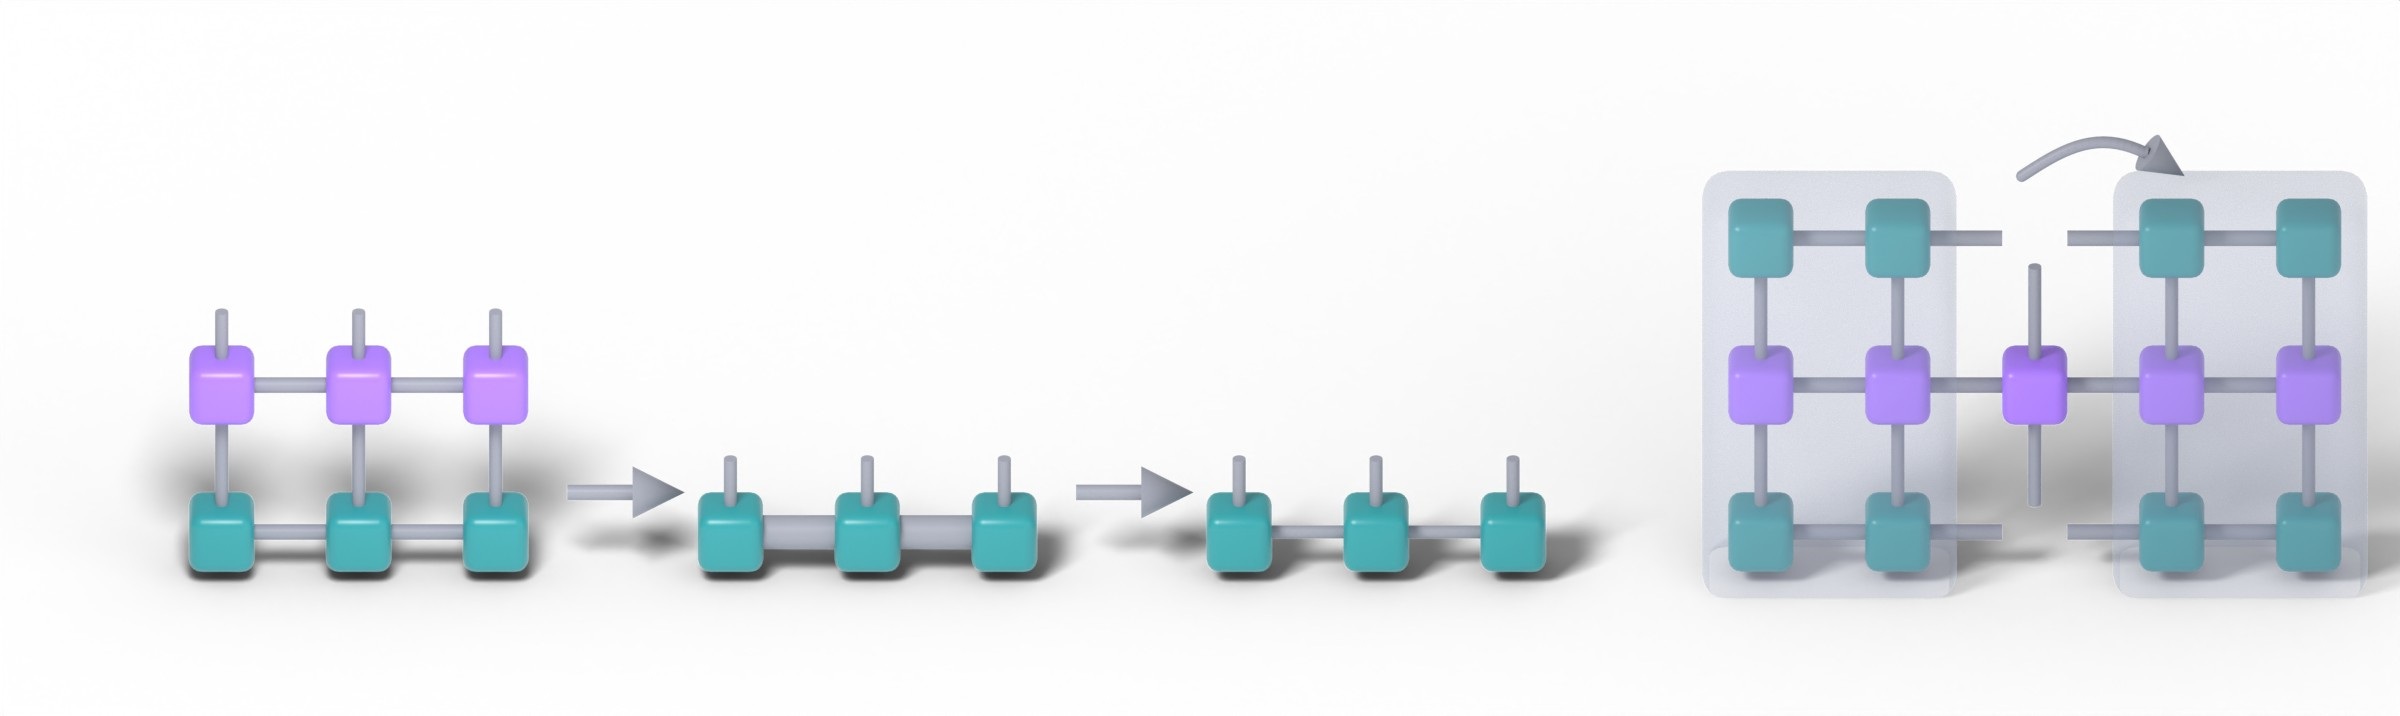
\includegraphics[width=\figw]{../blender/out/mps_algorithm.jpg}};
  %% written by figlib.py; x and y in units of the image width
\coordinate (chiS) at (0.0734\figw,0.0767\figw);
\coordinate (chiW) at (0.0734\figw,0.1379\figw);
\coordinate (HPsi) at (0.1495\figw,0.0555\figw);
\coordinate (chichiW) at (0.3899\figw,0.0626\figw);
\coordinate (svd) at (0.4728\figw,0.1002\figw);
\coordinate (chi) at (0.6019\figw,0.0626\figw);
\coordinate (L) at (0.7622\figw,0.0520\figw);
\coordinate (R) at (0.9334\figw,0.0520\figw);
\coordinate (site) at (0.8478\figw,0.0520\figw);
\coordinate (Mi) at (0.8543\figw,0.0767\figw);
\coordinate (sweep) at (0.9185\figw,0.2249\figw);
\coordinate (heff) at (0.8478\figw,0.2555\figw);
\coordinate (b) at (0.6766\figw,0.2932\figw);
\coordinate (a) at (0.0380\figw,0.2932\figw);

  \node[lbl, font=\normalsize, anchor=west] at (a) {(a)};
  \node[lbl, font=\normalsize, anchor=west] at (b) {(b)};
  \node[lbl, anchor=east] at (chiS) {$\chi$};
  \node[lbl, anchor=east] at (chiW) {$\chi_W$};
  \node[lbl, anchor=north] at (HPsi) {$\mathcal{H}\ket{\Psi}$};
  \node[lbl, anchor=north] at (chichiW) {$\chi\chi_W$};
  \node[lbl, anchor=south] at (svd) {SVD};
  \node[lbl, anchor=north] at (chi) {$\chi$};
  \node[lbl, anchor=north, align=center] at (L) {left\\environment};
  \node[lbl, anchor=north, align=center] at (R) {right\\environment};
  \node[lbl, anchor=north] at (site) {$i$};
  \node[lbl, anchor=west] at (sweep) {sweep};
  \node[lbl, anchor=west] at (Mi) {$M_i$};
  \node[lbl, anchor=south] at (heff) {$H_{\mathrm{eff}}(i)\,M_i^{s_i}=\lambda M_i^{s_i}$};
\end{tikzpicture}
\end{document}
